\section{Design and Analysis Modeling}
\label{sec:design_and_analysis_modelling}
We have four main systems, such as production management system, supply chain management system, communication management system, and availability management system. But among them, we are focusing only on the production management system and its features. There are multiple ways to represent software architectures, which can be seen in \ref{SysMLDiagram}. The proposed system for the architecture is illustrated in \ref{Featuremodel}. In this system, we have a production control system and a monitoring system where the first one contains operation and inventory features and the last one have logging and operational status features.

\begin{figure}[h]
\centering
  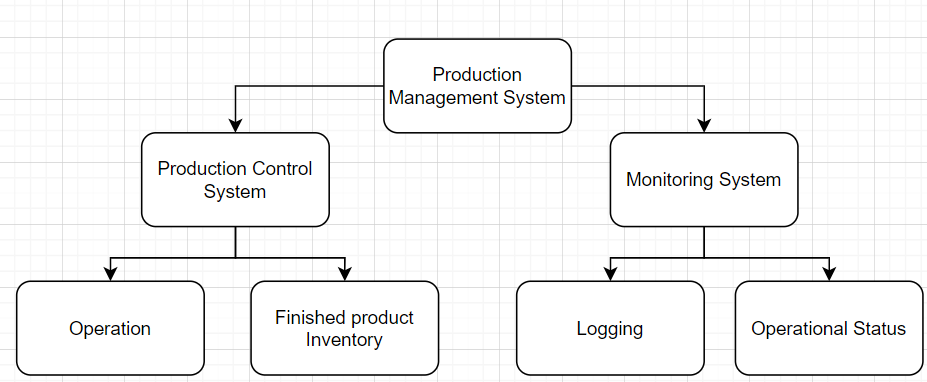
\includegraphics[width=\linewidth]{images/featuremodel.png}
  \caption{Feature model of the system}
  \label{Featuremodel}
\end{figure}

If we explore deep inside our block definition diagram (BDD), we have three main components \ref{fig:boat1}. They are Human Machine Interface (HMI), communication middleware (Bus), and automated guided cart (AGC). To support those components, we have a database component for logging the events. The main function of our HMI is to orchestrate stimulus from the environment and translate those signals through the functional block “Controller” for various purposes. For example, in our use case one, the production manager wants to start operation, so he interacts with the HMI through a start button and the controller generates a message to publish this information to the bus and the AGC, which is subscribed to this bus, receives the data, logs an acknowledgment to the database, and simultaneously initiates its operation for the production. 

\begin{figure}[h]
\centering
  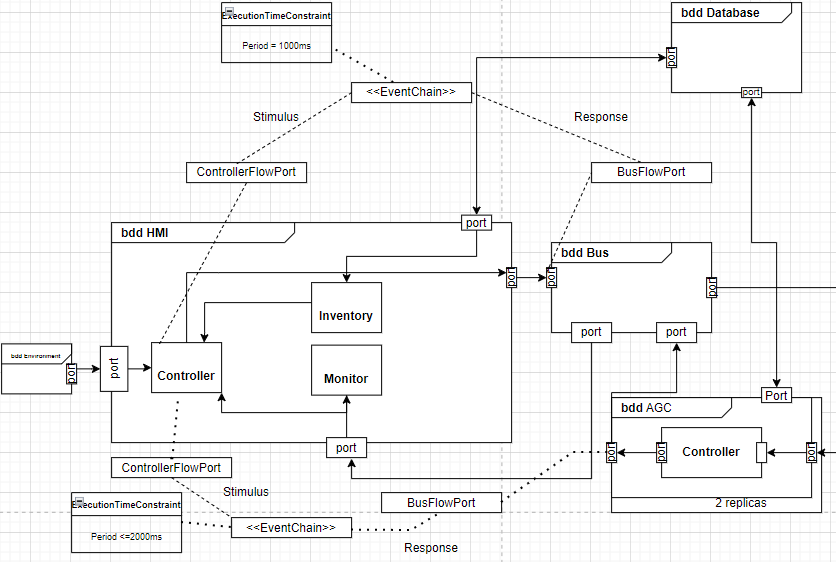
\includegraphics[width=\linewidth]{images/structuremodel2.png}
  \caption{Structure of the system}
  \label{fig:boat1}
\end{figure}

There are different programming languages that have their own merits and advantages for various developments. We select two different programming languages for our two software interacting interfaces. For HMI, we are going with next.js as it is full-stack and it has a clear advantage to make UI components using react.js as well as a backend feature. On the other hand, for the AGC, a lightweight and integrable programming language was highly desirable. Python has all of those qualities, as well as easy syntax with a strong community. Although performance might be a hindrance, we trade off this quality with others. When we are selecting our database for our logging and inventory management, we are looking for ACID compliant (Atomicity, Consistency, Isolation, Durability) and PostgreSQL is perfect for this as it also ensures data integrity and reliability, which can be critical for an inventory tracking system. For choosing the message bus, there was a lot of different benefits between Apache Kafka, pure MQTT, RabbitMQ and more. In the end we selected RabbitMQ as it has both AMQP and MQTT features, and it is lightweight with compared to Apache Kafka.

\begin{table}[h]
\begin{tabular}{|p{1cm}|p{7cm}|}
\hline
ID & Description \\
\hline
Req\#1 & The system will provide a button for the production manager(user) where the manager will start production, the HMI will take this as an action for producing signals to other components to start working. \\
\hline
Req\#2 & The HMI controller will generate a message for publication. \\
\hline
Req\#3 & The HMI controller will publish the generated message to the BUS system which transmits this message to all components in less than 1 second. \\
\hline
Req\#3.1 & Log the operation’s information for the product into the database. \\
\hline
Req\#4 & The AGC component will receive the message from HMI controller within 2 Sec. \\
\hline
Req\#4.1 & Log the operation’s receiving information for the product into database. \\
\hline
Req\#5 & After receiving the "start production" message, AGC will start its production. \\
\hline
Req\#6 & After completing a task, AGC will publish a message indicating it has finished. \\
\hline
Req\#6.1 & Log AGC task completion of the production into the database. \\
\hline
Req\#7 & HMI will receive the quantity of the product and completes the production. \\
\hline
\end{tabular}
\caption{Requirement table}
\label{tab:req_table}
\end{table}

According to our top-level requirements \ref{tab:req_table}, we have emphasized our attention in two main quality attributes (QAs), one is availability and the other are integrability. There are certain points behind these QAs. Availability refers to the system's uptime for its core functionality all the time and it builds on the concept that whenever a system is down it will recover itself through different means as it seems it masks the faults as if it never happened. It is closely related to performance but differs when the system has failed, as the system will still be available but might respond more slowly. It is also closely related to safety as it prevents a system from entering a hazardous state or limiting damage when it does, and lastly closely but clearly distinct from security\cite{bass2021software}. For achieving availability we use the active redundancy pattern and Docker, which helps us to achieve this as it ensures if any faults occur then Docker will use redundant spare. The benefit of this pattern is that it requires a brief delay in the presence of a failure where the alternative would require the system to stop and repair it which would take hours or days. The downside of its cost and complexity. 

We chose integrability as our other QA keeping in mind that we need to integrate different components in our system and use a communication bus. We prefer to decouple our components so that we could add more components with different types more easily and without any dependency. However, to achieve this quality we have to tradeoff performance but it could help us modify it more easily which is our future plan. For achieving this QA, we use orchestration tactics as our HMI is the main coordinator. It collects information and publishes and receives information from other components like AGC through our message bus RabbitMQ. One of the main problems of this tactic is if our bus system is crushed then the whole system will break down, and to overcome this we use Docker containers for our bus with replication. 
